\documentclass{article}

\textheight 22.5truecm \textwidth 14.5truecm
\setlength{\oddsidemargin}{0.35in}\setlength{\evensidemargin}{0.35in}

\setlength{\topmargin}{-.5cm}
\usepackage[utf8]{inputenc}
\usepackage[russian]{babel}
\usepackage{graphicx}
\usepackage{amsmath}
\usepackage{breqn}
\usepackage{wrapfig}
\usepackage{float}
\usepackage{multirow}
\usepackage{caption}
\usepackage{subcaption}
\usepackage{textcomp}

\graphicspath{ {./data/images} }
\author{Александр Романов Б01-110}
\date{}
\title{5.5.5 Компьютерная сцинтилляционная $\gamma$-спектроскопия}

\begin{document}
\maketitle
\section{Работа}
Включим компьютер и питание экспериментальной установки. Будем располагать измеряемые образцы в 
сцинтилляционном счётчике, запускать измерение и ждать пока на экране не появится чёткая картина пиков,
связанных с фотоэффектом, эффектом Комптона и т.д. Результаты сохраним.
\section{Обработка результатов}
\subsection{Co60}
Приведём результаты измерений для \(Co60\).

\begin{figure}[H]
	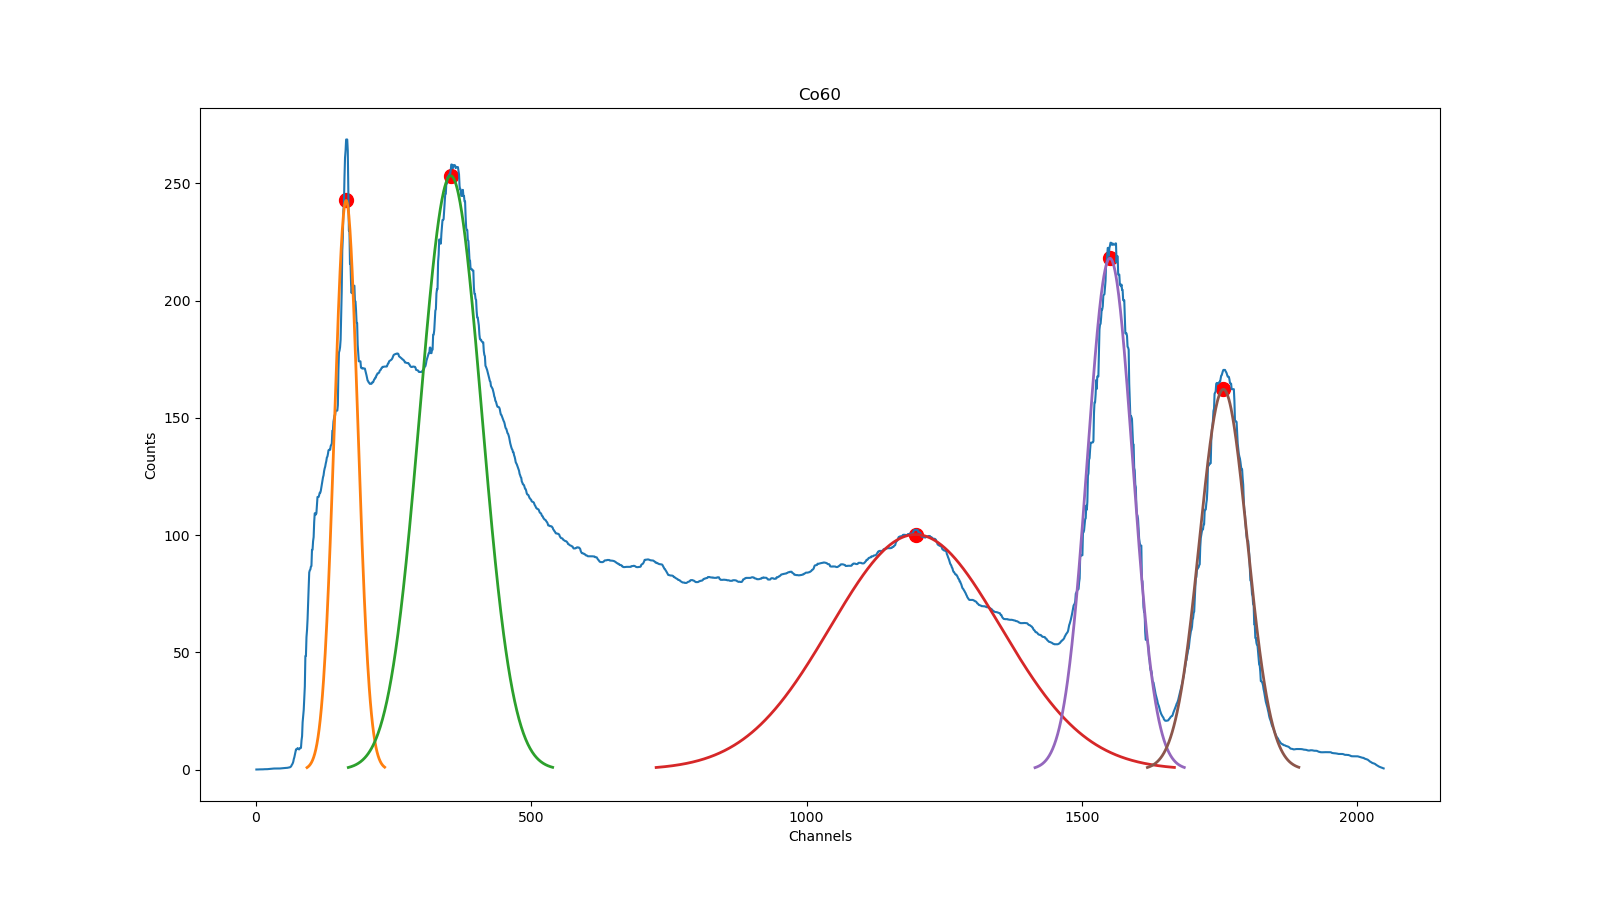
\includegraphics[width=\textwidth]{Co60.png}
\end{figure}

Сведём информацию о положении пиков в таблицу

\begin{table}[H]
	\centering
	\begin{tabular}{|c|c|c|c|c|c|}
		\hline
		Peak \(N\textsuperscript{\underline{o}}\)& 1 & 2 & 3 & 4 & 5 \\\hline
		Channel & 164 & 354 & 1198 & 1551 & 1757\\\hline
		Count   & 242 & 253 & 100 & 218 & 162\\\hline
	\end{tabular}
\end{table}

Сопоставим каждому пику табличные значения энергии для фотопиков:

\begin{table}[H]
	\centering
	\begin{tabular}{|c|c|c|}
		\hline
		Channel       & 1551  & 1757 \\\hline
		Energy, MeV   & 1.173 & 1.332\\\hline
	\end{tabular}
\end{table}

\subsection{Cs137}
Приведём результаты измерений для \(Cs137\).

\begin{figure}[H]
	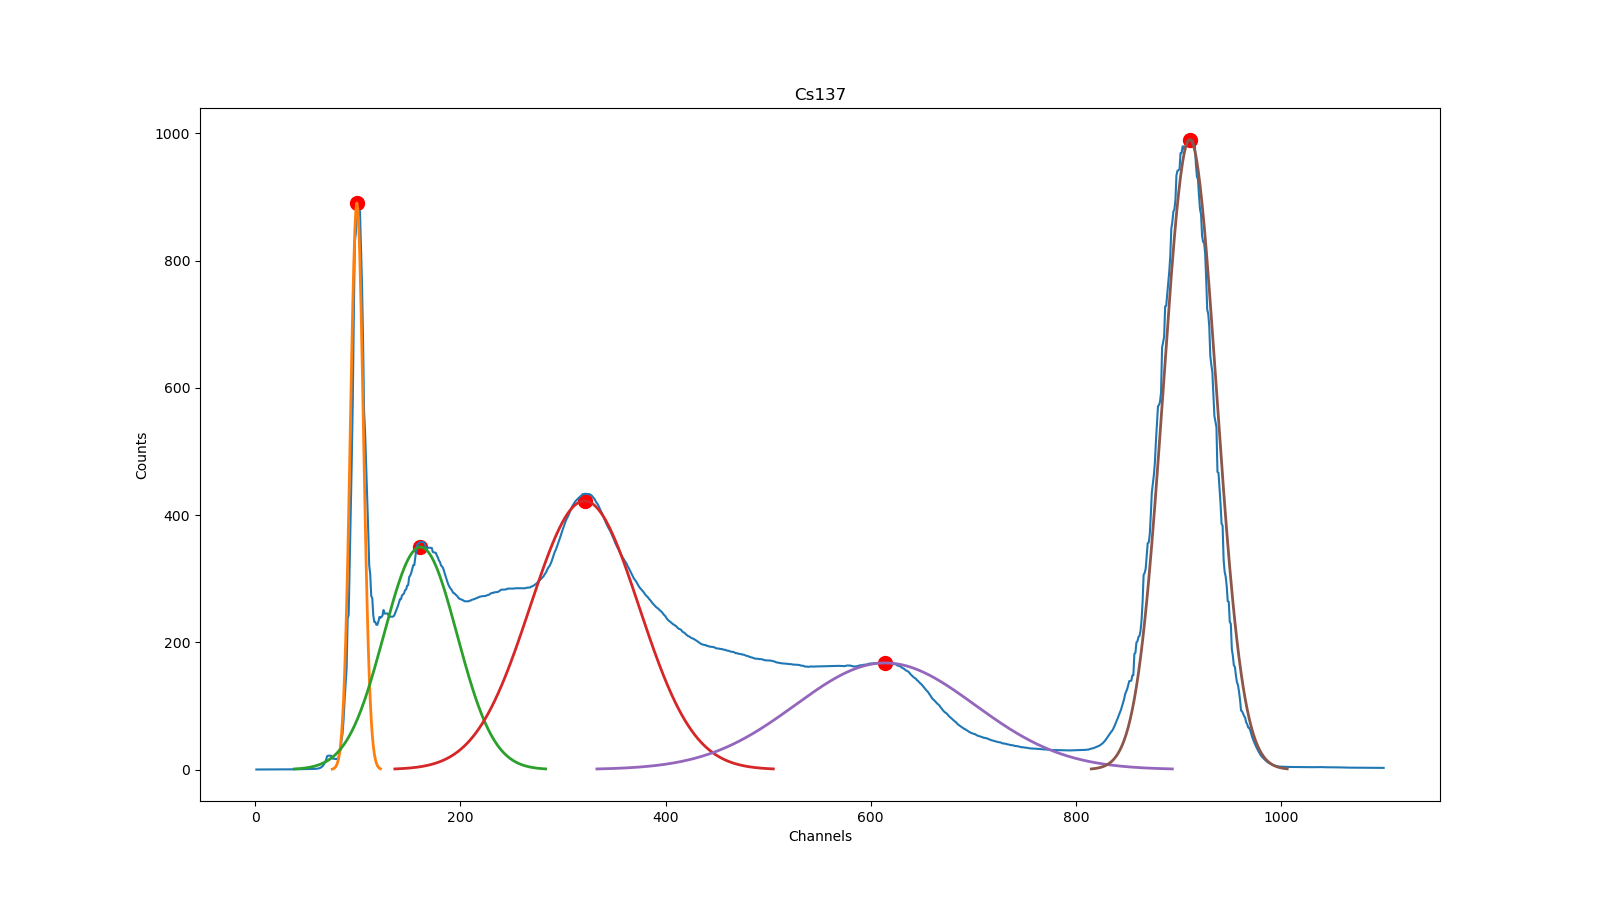
\includegraphics[width=\textwidth]{Cs137.png}
\end{figure}

Сведём информацию о положении пиков в таблицу

\begin{table}[H]
	\centering
	\begin{tabular}{|c|c|c|c|c|c|}
		\hline
		Peak \(N\textsuperscript{\underline{o}}\)& 1 & 2 & 3 & 4 & 5 \\\hline
		Channel & 99 & 161 & 321 & 614 & 911 \\\hline
		Count   & 890 & 349 & 422  & 167 & 990\\\hline
	\end{tabular}
\end{table}

Сопоставим каждому пику табличные значения энергии для фотопика:

\begin{table}[H]
	\centering
	\begin{tabular}{|c|c|}
		\hline
		Channel       & 911    \\\hline
		Energy, MeV   & 0.6617 \\\hline
	\end{tabular}
\end{table}

\subsection{Na22}
Приведём результаты измерений для \(Na22\).

\begin{figure}[H]
	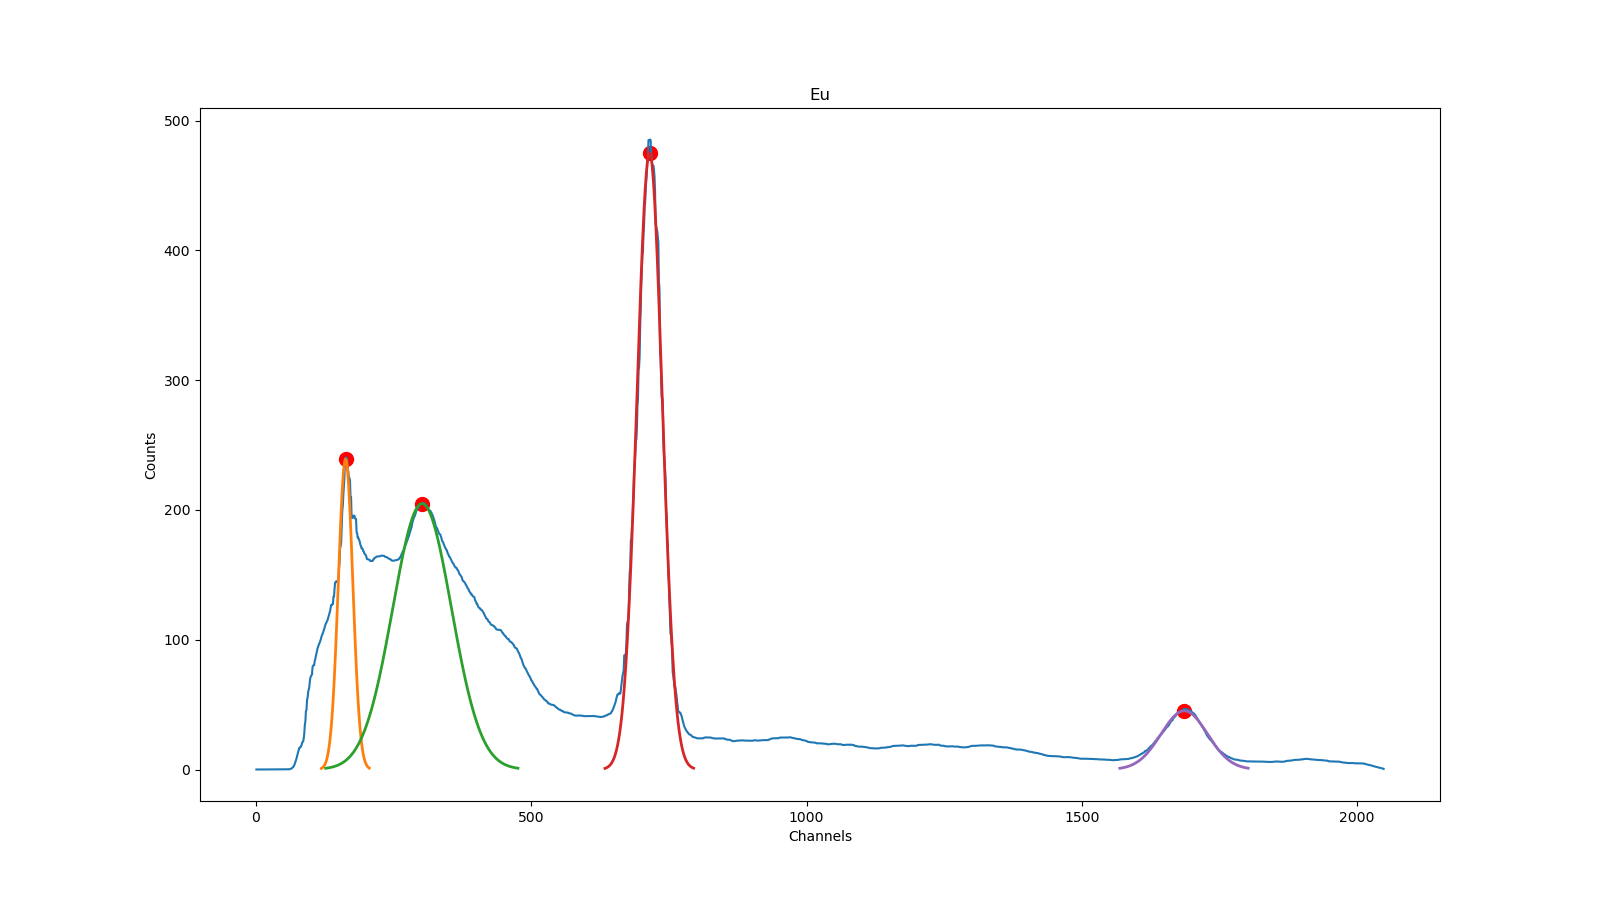
\includegraphics[width=\textwidth]{na22.png}
\end{figure}

Сведём информацию о положении пиков в таблицу

\begin{table}[H]
	\centering
	\begin{tabular}{|c|c|c|c|c|}
		\hline
		Peak \(N\textsuperscript{\underline{o}}\)& 1 & 2 & 3 & 4 \\\hline
		Channel & 163 & 302 & 715 & 1686 \\\hline
		Count   & 239 & 204 & 475 & 45 \\\hline
	\end{tabular}
\end{table}
\subsection{Eu}
Приведём результаты измерений для \(Eu\).

\begin{figure}[H]
	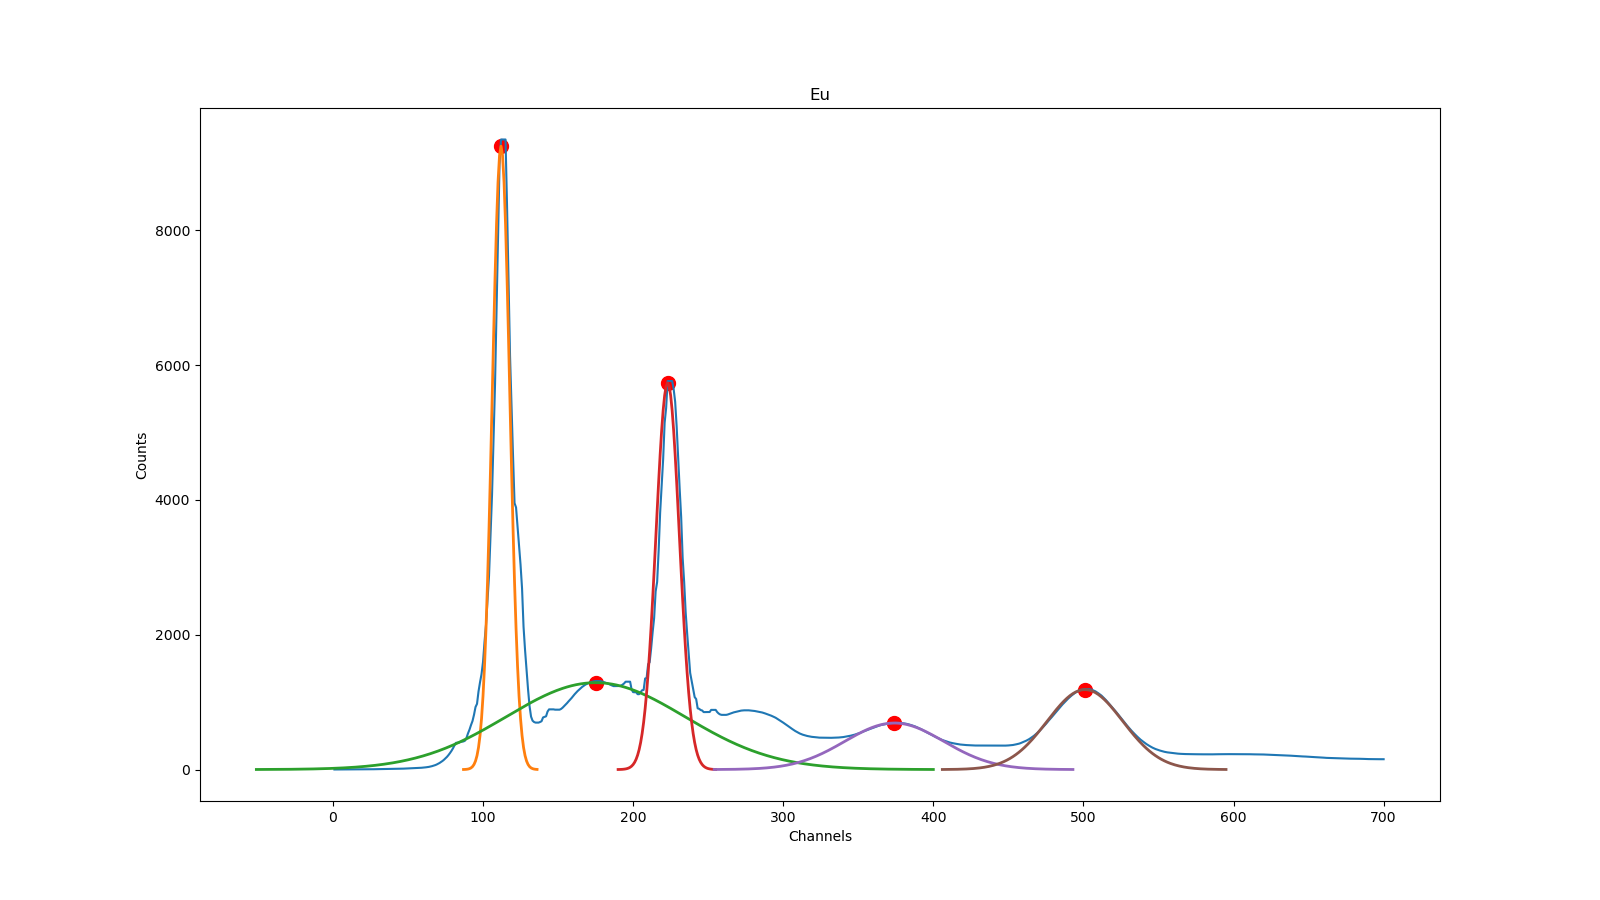
\includegraphics[width=\textwidth]{Eu.png}
\end{figure}

Сведём информацию о положении пиков в таблицу

\begin{table}[H]
	\centering
	\begin{tabular}{|c|c|c|c|c|c|c|}
		\hline
		Peak \(N\textsuperscript{\underline{o}}\)& 1 & 2 & 3 & 4 & 5 & 6\\\hline
		Channel & 112 & 175 & 223 & 274 & 374 & 501\\\hline
		Count   & 9248 & 1288 & 5736 & 878 & 690 & 1185 \\\hline
	\end{tabular}
\end{table}

\subsection{Am}
Приведём результаты измерений для \(Am\).

\begin{figure}[H]
	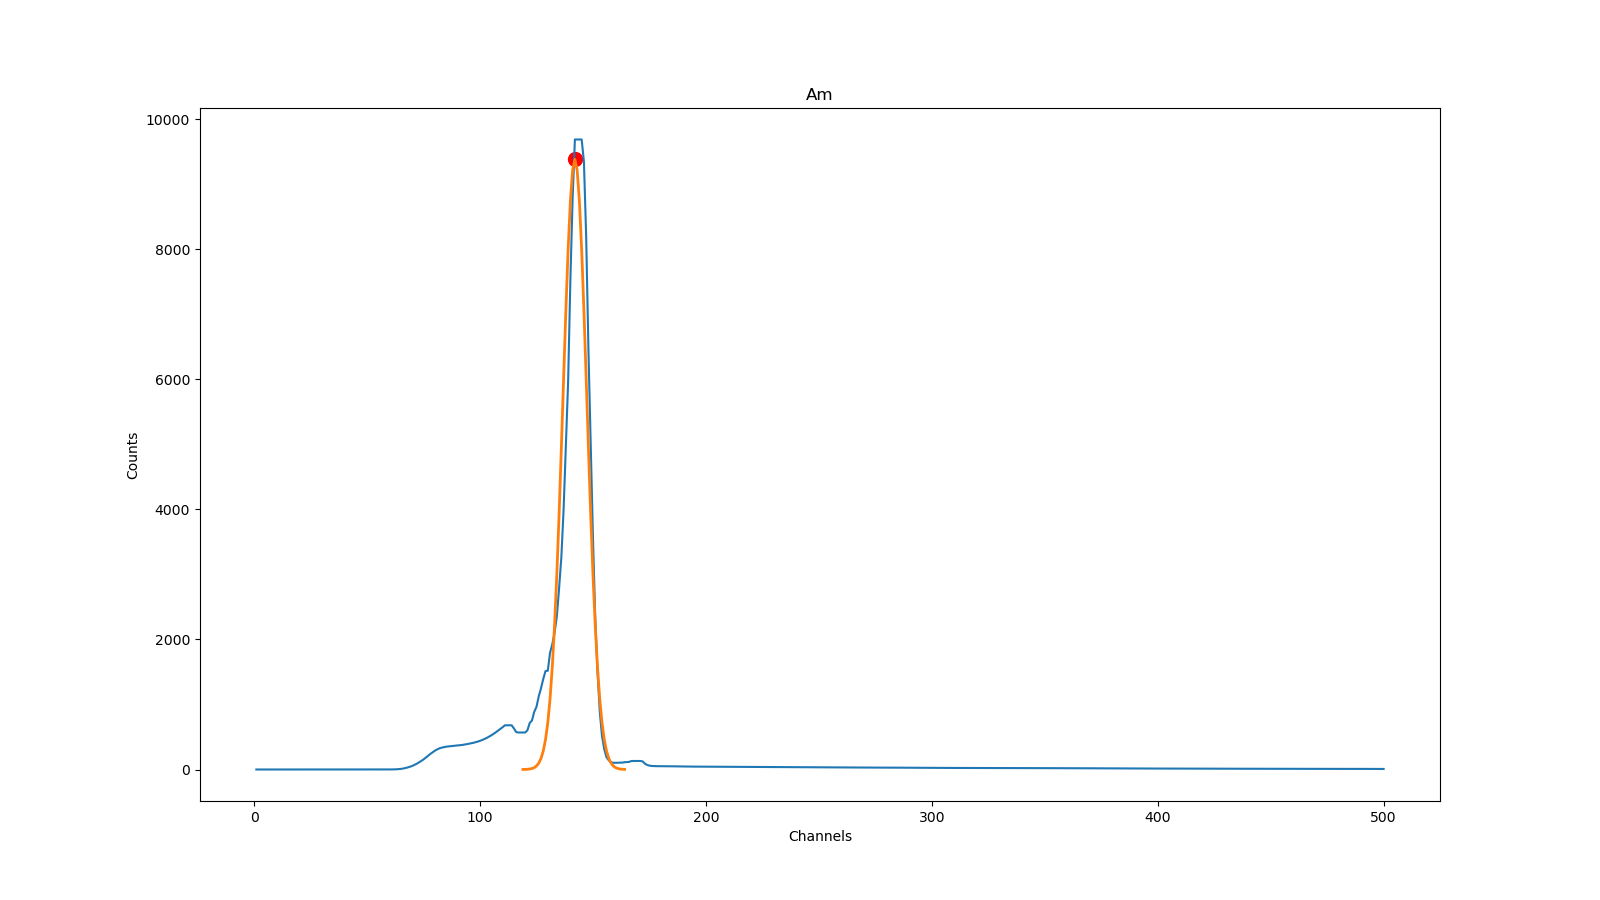
\includegraphics[width=\textwidth]{Am.png}
\end{figure}

Сведём информацию о положении пиков в таблицу

\begin{table}[H]
	\centering
	\begin{tabular}{|c|c|}
		\hline
		Peak \(N\textsuperscript{\underline{o}}\)& 1\\\hline
		Channel & 142 \\\hline
		Count   & 9384 \\\hline
	\end{tabular}
\end{table}

\subsection{Фотопики}
Сведём информацию о фотопиках \(Co60\) и \(Cs137\) в одну таблицу:

\begin{table}[H]
	\centering
	\begin{tabular}{|c|c|c|c|}
		\hline
		Channel     & 1551  & 1757  & 911\\\hline
		Energy, MeV & 1.173 & 1.332 & 0.6617 \\\hline
	\end{tabular}
\end{table}
Проведём апроксимацию:

\begin{figure}[H]
	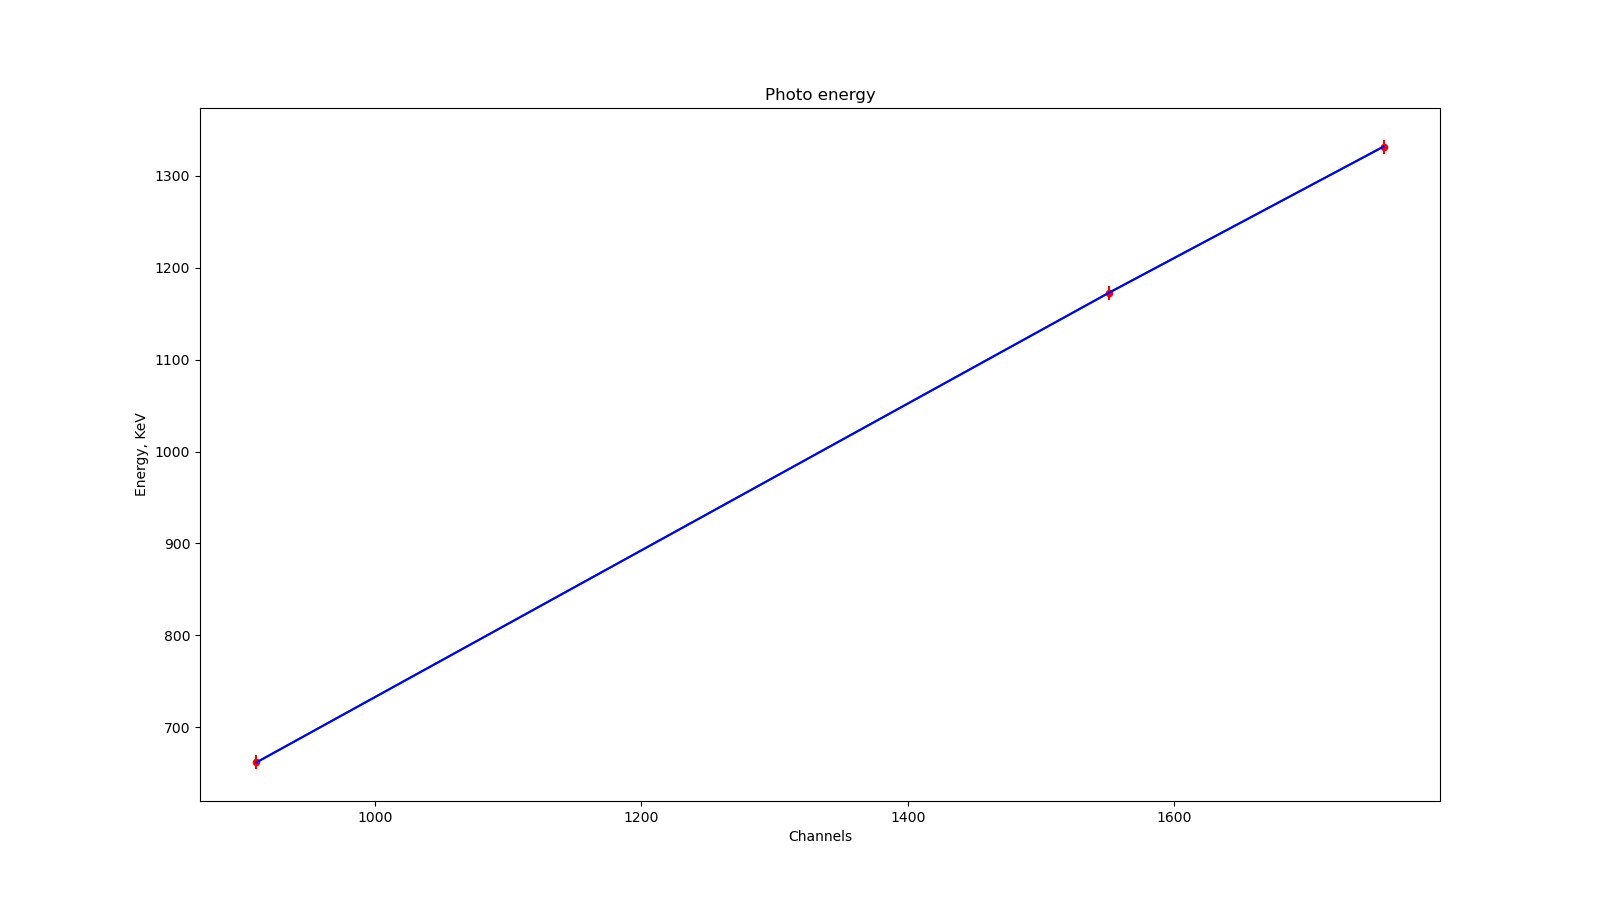
\includegraphics[width=\textwidth]{channel-energy.png}
\end{figure}

\[E = (0.79 \pm 0.005\;KeV)\cdot N-(60.9 \pm 7.86\;KeV)\]
Согласно результатам этой апроксимации можно вычислить значение энергии фотопиков для
\(Na22\) и \(Eu\):

\[E_{Na22} = 0.79 \cdot 1686 - 60.9 = 1270 \pm 16\; KeV \]
\[E_{Eu_1} = 0.79 \cdot 374 - 60.9 = 235 \pm 10\; KeV  \]
\[E_{Eu_2} = 0.79 \cdot 501 - 60.9 = 334 \pm 10\; KeV  \]

Сведём энергии фотопиков всех веществ в одну таблицу:
\begin{table}[H]
	\centering
	\begin{tabular}{|c|c|c|c|c|}
		\hline
		Metal       & Cs137 & Co60  & Na22 & Eu\\\hline
		Channel     & 911   & 1551  & 1686 & 501\\\hline
		Energy, KeV & 662   & 1332  & 1270 & 334\\\hline
	\end{tabular}
\end{table}
\subsection{Зависимость энергии пиков обратного рассеяния от фотопиков}

Сведём в одну таблицу значения энергий пиков обратного рассеяния для всех образцов
\begin{table}[H]
	\centering
	\begin{tabular}{|c|c|c|c|c|}
		\hline
		Metal       & Cs137& Co60 & Na22 & Eu   \\\hline
		Channel     & 161   & 354  & 302  & 223 \\\hline
		Energy, KeV & 66    & 218  & 178  & 115 \\\hline
	\end{tabular}
\end{table}


Построим зависимость энергии пиков полного отражение от энергии фотопиков:
\begin{figure}[H]
	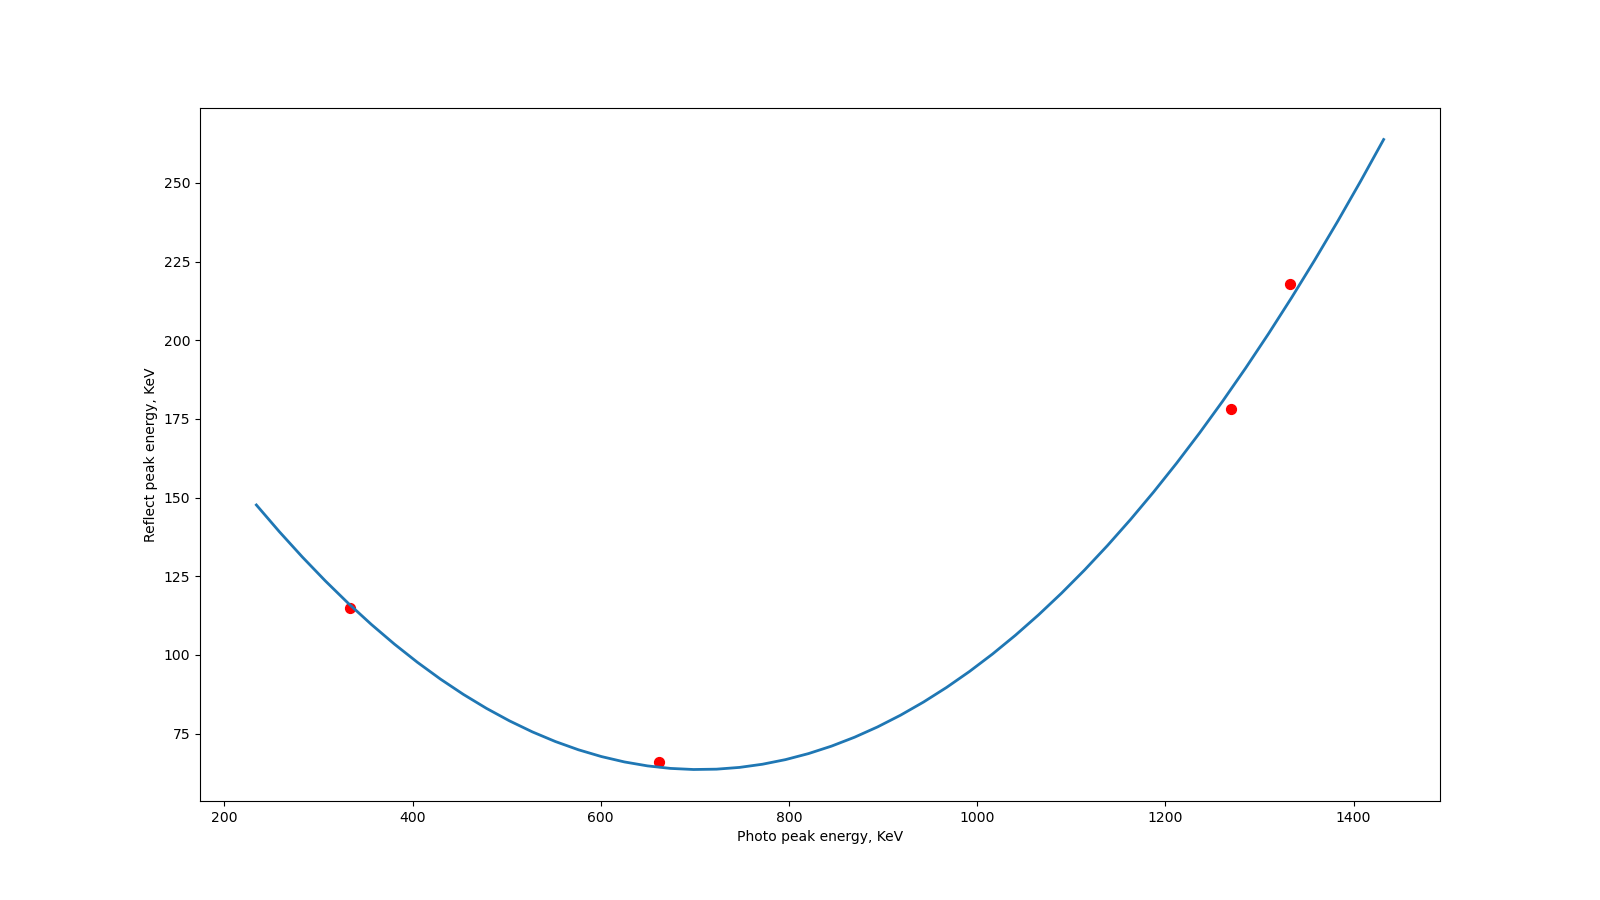
\includegraphics[width=\textwidth]{photo-reflect.png}
\end{figure}

\section{Выводы}
В ходе выполнения работы:
\begin{enumerate}
	\item Были исследованы спектры излучения различных радиоактивных веществ.
	\item Были изучены положения различных пиков: фотопиков, краёв комптоновского поглощения,
		обратного отражения и другие.
\end{enumerate}
\end{document}
